\documentclass[tikz]{standalone}

\usepackage[latin1]{inputenc}
\usepackage{tikz}

% GNUPL
\begin{document}
\pagestyle{empty}


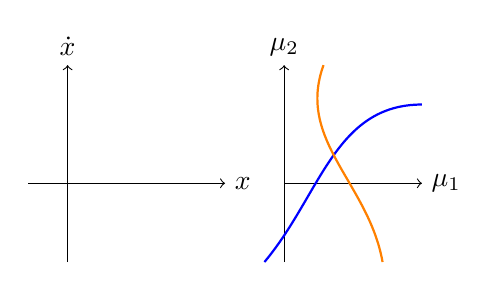
\begin{tikzpicture}[scale=0.5]
    %\draw[very thin,color=gray] (-1,1.1) grid (3.9,3.9);
    \draw[->] (-1,0) -- (4,0) node[right] {$x$};
    \draw[->] (0,-2) -- (0,3) node[above] {$\dot x$};
    \draw[->] (5.5,0) -- (9,0) node[right] {$\mu_1$};
    \draw[->] (5.5,-2) -- (5.5,3) node[above] {$\mu_2$};
    \draw[blue,thick] (5,-2) to [out=50,in=180] (9,2);  
    \draw[orange,thick] (6.5,3) to [out=-110,in=100] (8,-2);  
\end{tikzpicture}


\end{document}